
%(BEGIN_QUESTION)
% Copyright 2006, Tony R. Kuphaldt, released under the Creative Commons Attribution License (v 1.0)
% This means you may do almost anything with this work of mine, so long as you give me proper credit

Examine this microcontroller circuit and program, designed to act as a general-purpose proportional controller:

$$\includegraphics[width=15.5cm]{i01486x01.eps}$$

\hbox{ \vrule
\vbox{ \hrule \vskip 3pt
\hbox{ \hskip 3pt
\vbox{ \hsize=5in \raggedright

\noindent
\underbar{\bf Pseudocode listing}

\vskip 10pt

{\tt Declare Pin0 as an analog input (scale 0 to 5 volts = 0 to 1023)}

{\tt Declare Pin1 as an analog output (scale 0 to 5 volts = 0 to 1023)}

{\tt Declare SP as a variable, initially set to a value of 614}

{\tt Declare GAIN as a variable, initially set to a value of 1.0}

{\tt Declare ERROR as a variable}

{\tt Declare BIAS as a constant = 614}

\vskip 10pt

{\tt LOOP}

\hskip 10pt {\tt SET ERROR = Pin0 - SP}

\hskip 10pt {\tt SET Pin1 = (GAIN * ERROR) + BIAS}

{\tt ENDLOOP}
}
\hskip 3pt}%
\vskip 5pt \hrule}%
\vrule}


\vskip 10pt

Is this controller {\it direct} or {\it reverse} acting?  What edit(s) to the program listing would be required to change the direction of the controller's action?  

\vskip 20pt \vbox{\hrule \hbox{\strut \vrule{} {\bf Suggestions for Socratic discussion} \vrule} \hrule}

\begin{itemize}
\item{} Which sections of the pseudocode program listing are executed repeatedly, and which sections are executed only once?
\item{} How many bits of resolution does this microcontroller have for the analog input on pin \#1, assuming that 0 to 1023 is the full range of the converter?
\item{} Does the speed of program execution (i.e. how fast the loop repeats itself) affect the controller's ability to control a process?
\item{} Could all the ``Declare'' instructions be placed within the loop of this program?  Why or why not?
\item{} Explain what would happen if you deleted the {\tt LOOP} and {\tt ENDLOOP} statements in the microcontroller program.
\item{} Modify this program to include a PV alarm, turning on an LED alarm lamp if the PV exceeds a certain value, and turning it back off when the PV drops below another value.
\end{itemize}


\underbar{file i01486}
%(END_QUESTION)





%(BEGIN_ANSWER)

The controller code as shown implements {\it direct} action, since the error is calculated as PV $-$ SP.

\vskip 10pt

The following additions give this controller the ability to switch between direct or reverse control action:

$$\includegraphics[width=15.5cm]{i01486x02.eps}$$

\hbox{ \vrule
\vbox{ \hrule \vskip 3pt
\hbox{ \hskip 3pt
\vbox{ \hsize=5in \raggedright

\noindent
\underbar{\bf Pseudocode listing}

\vskip 10pt

{\tt Declare Pin0 as an analog input (scale 0 to 5 volts = 0 to 1023)}

{\tt Declare Pin1 as an analog output (scale 0 to 5 volts = 0 to 1023)}

{\tt Declare Pin7 as a discrete input}

{\tt Declare SP as a variable, initially set to a value of 614}

{\tt Declare GAIN as a variable, initially set to a value of 1.0}

{\tt Declare ERROR as a variable}

{\tt Declare BIAS as a constant = 614}

\vskip 10pt

{\tt LOOP}

\hskip 10pt {\tt IF Pin7 = 0, SET ERROR = Pin0 - SP }

\hskip 10pt {\tt ELSE, SET ERROR = SP - Pin0}

\hskip 10pt {\tt ENDIF}

\vskip 10pt

\hskip 10pt {\tt SET Pin1 = (GAIN * ERROR) + BIAS}

{\tt ENDLOOP}
}
\hskip 3pt}%
\vskip 5pt \hrule}%
\vrule}


\vskip 10pt

While a very slow program execution time could be bad for control, it actually could serve a useful purpose in some processes.  In processes with large dead times (transport delays), one control strategy to apply is called {\it sample-and-hold}, which is precisely what this program would be if a purposeful and substantial delay time were inserted into the loop.

%(END_ANSWER)





%(BEGIN_NOTES)

\vfil \eject

\noindent
{\bf Summary Quiz:}

Determine whether this digital control program is {\it direct-acting} or {\it reverse-acting}:

\vskip 10pt

\hbox{ \vrule
\vbox{ \hrule \vskip 3pt
\hbox{ \hskip 3pt
\vbox{ \hsize=5in \raggedright

\noindent
\underbar{\bf Pseudocode listing}

\vskip 10pt

{\tt Declare Pin0 as an analog input (scale 0 to 5 volts = 0 to 1023)} {\it (PV)}

{\tt Declare Pin1 as an analog output (scale 0 to 5 volts = 0 to 1023)}

{\tt Declare SP as a variable, initially set to a value of 512}

{\tt Declare GAIN as a variable, initially set to a value of 1.0}

{\tt Declare ERROR as a variable}

{\tt Declare BIAS as a constant = 512}

\vskip 10pt

{\tt LOOP}

\hskip 10pt {\tt SET Pin1 = (GAIN * (SP - Pin0)) + BIAS}

{\tt ENDLOOP}
}
\hskip 3pt}%
\vskip 5pt \hrule}%
\vrule}

%INDEX% Control, proportional: digital electronic controller

%(END_NOTES)


